\documentclass[11pt,compress,t,notes=noshow, aspectratio=169, xcolor=table]{beamer}

\usepackage[nospeakermargin]{../../style/lmu-lecture-2}
% Defines macros and environments
\input{../../style/common.tex}
\usepackage{pax}
\setbeamertemplate{frametitle}{\expandafter\uppercase\expandafter\insertframetitle}
%\useoutertheme{metropolis}
% remove section slides
\AtBeginSection[]
{
	\begin{frame}<beamer>
		\frametitle{Advanced Machine Learning}
		\tableofcontents[currentsection]
	\end{frame}
}
% includepdf slides, pagecommad will set counter for framenumber
\usepackage{pdfpages}
\includepdfset{trim=0mm 0mm 0mm 0mm, pagecommand={\global\setcounter{framenumber}{\value{page}}}}
% trim=0mm 6mm 0mm 0mm, offset=0 15,
% add footer:
\usepackage{framed, color}
\usepackage{xcolor}
%\iffalse
\setbeamertemplate{footline}[text line]{%
	\noindent\hspace*{\dimexpr-\oddsidemargin-1in\relax}%
	\colorbox{white}{
		\makebox[\dimexpr\paperwidth-2\fboxsep\relax]{
			\color{black}
			\begin{minipage}[c][2ex][c]{0.5\linewidth}
				\secname
			\end{minipage}
			\hfill\begin{minipage}[c][2ex][c]{0.5\linewidth}
				\flushright
				\insertframenumber{}~/~\inserttotalframenumber~~
			\end{minipage}
	}}%
	\hspace*{-\paperwidth}
}
%\fi
\title{Applied Machine Learning}
% \author{LMU}
%\institute{\href{https://compstat-lmu.github.io/lecture_iml/}{compstat-lmu.github.io/lecture\_iml}}
\date{}

\begin{document}

\newcommand{\titlefigure}{figure/empty}
\newcommand{\learninggoals}{
\item Categorical Encoding: \newline One-Hot and Target/Impact Encoding
\item Feature Transformations: \newline Normalization and Box-Cox Transformation
\item Intro to mlr3pipelines}

\lecturechapter{Feature Engineering}
\lecture{Applied Machine Learning}


\section{Introduction to Feature Engineering}
\includepdf[pages={3}]{pdf_chapters/slides_intro_fe.pdf}
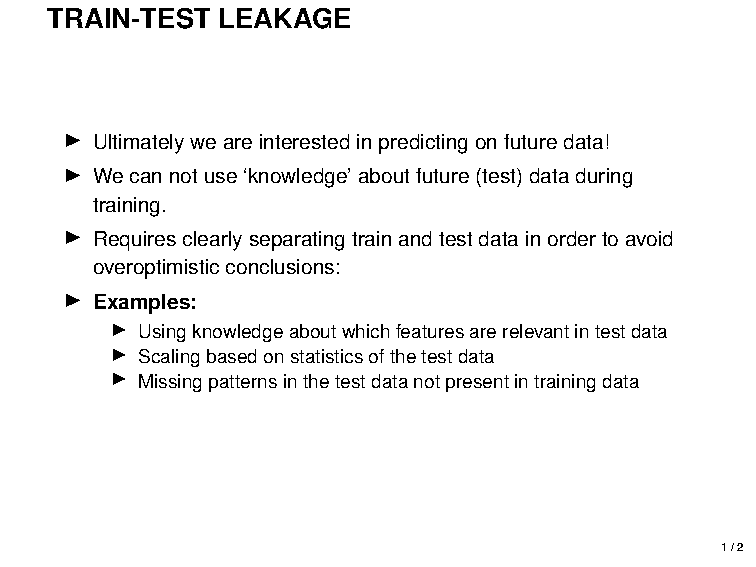
\includepdf[pages={1-last}]{pdf_chapters/slides_leakage.pdf}
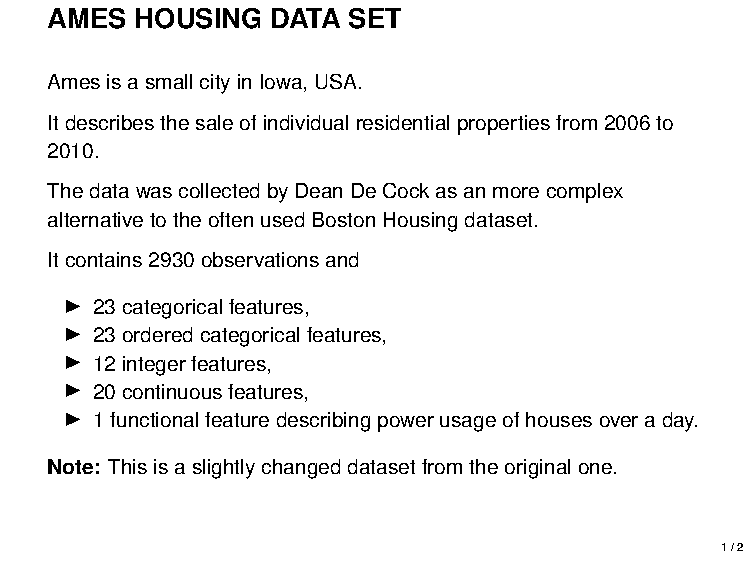
\includepdf[pages={1-last}]{pdf_chapters/slides_ames_extended.pdf}
\section{Handling of Categorical Features}
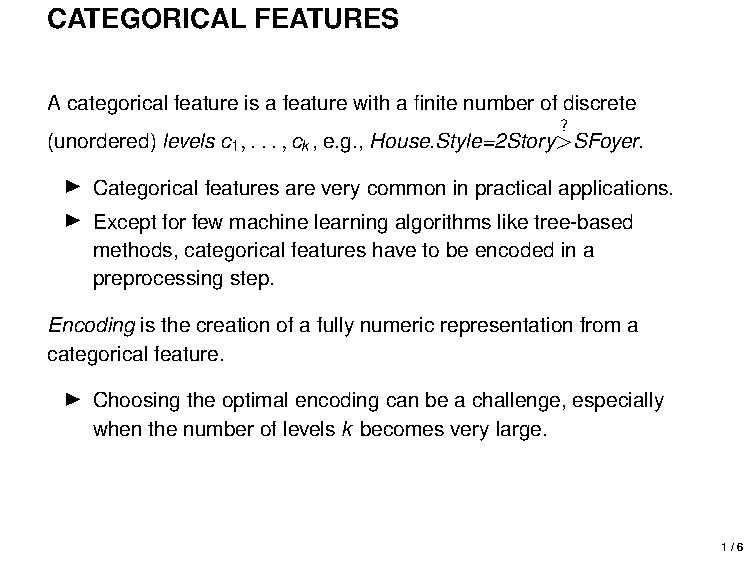
\includepdf[pages={1-4, last}]{pdf_chapters/slides_categ_encode_dummy.pdf}
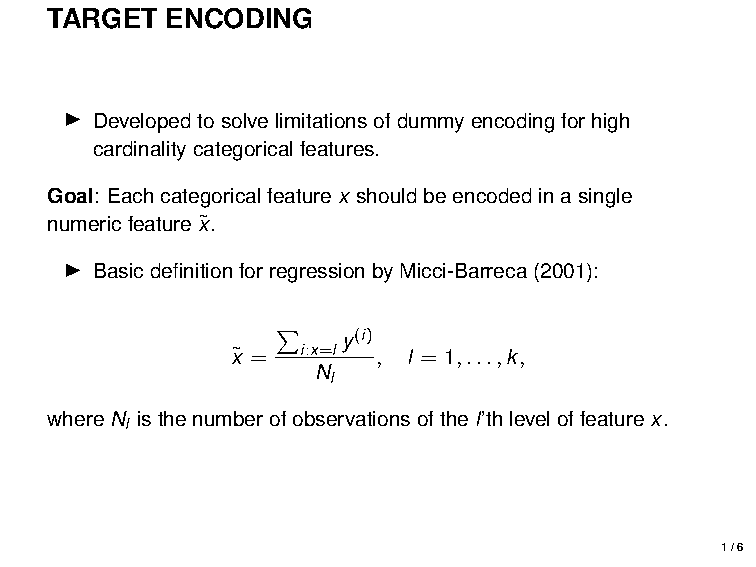
\includepdf[pages={1-last}]{pdf_chapters/slides_categ_encode_impact.pdf}
\section{Feature Transformation}
%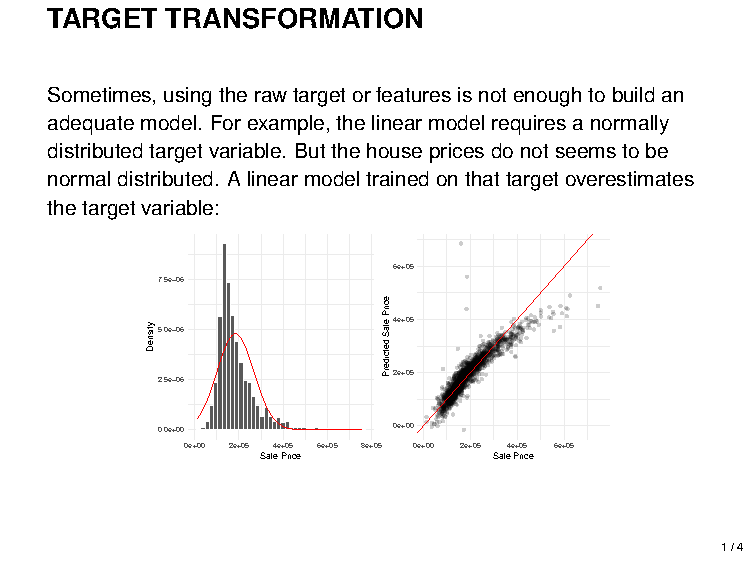
\includepdf[pages={1-last}]{pdf_chapters/slides_01_ftt_target.pdf}
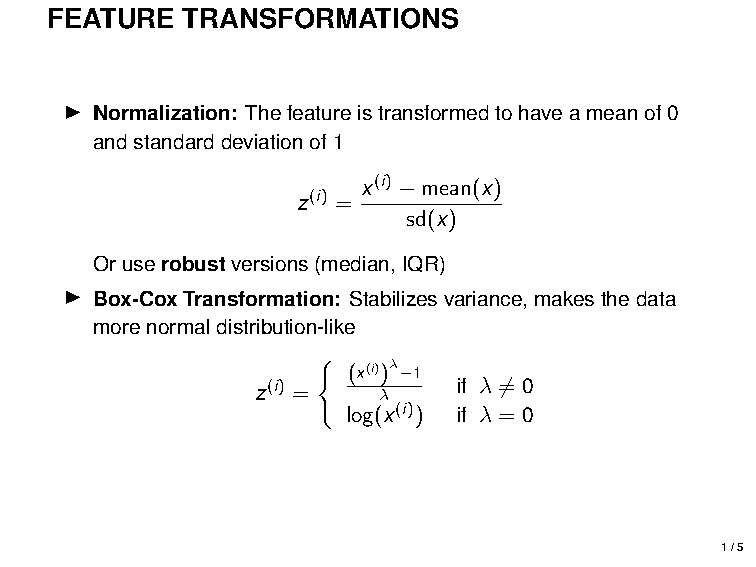
\includepdf[pages={1-last}]{pdf_chapters/slides_02_ftt_feature_trafos.pdf}
\section{Imputation}
\includepdf[pages={3-last}]{pdf_chapters/slides_01_imputation_intro.pdf}
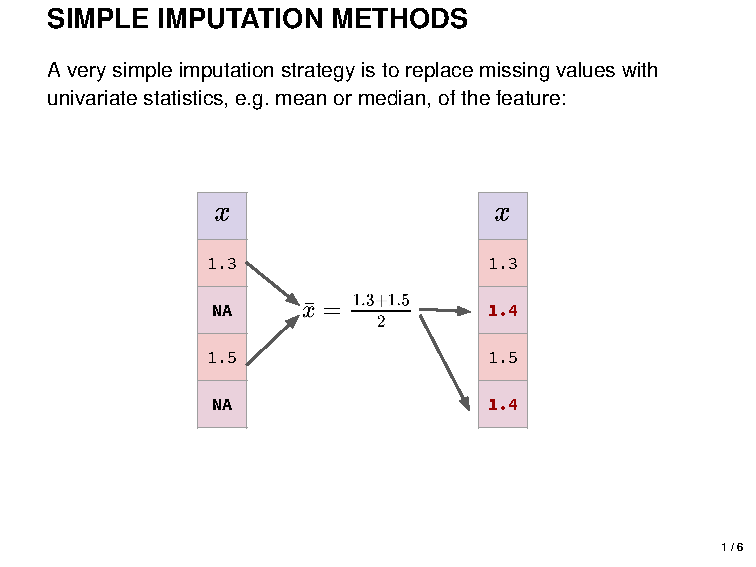
\includepdf[pages={1-5}]{pdf_chapters/slides_02_imputation_simple.pdf}
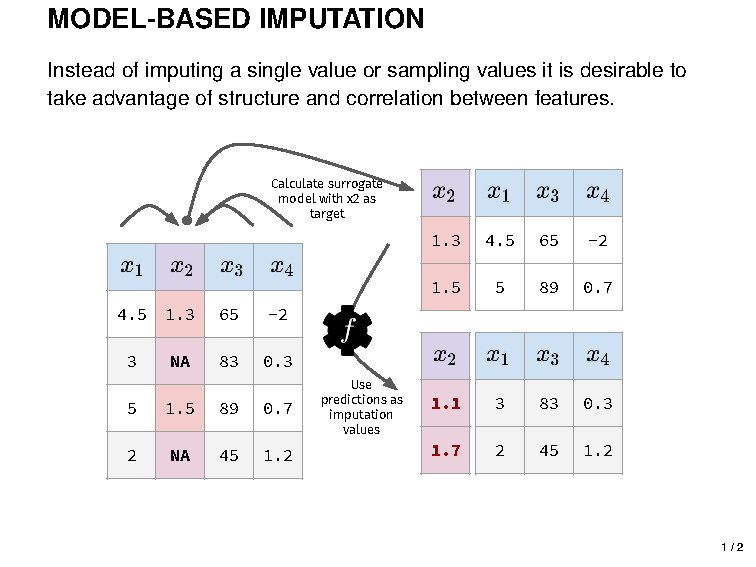
\includepdf[pages={1-last}]{pdf_chapters/slides_03_imputation_models.pdf}
\section{mlr3pipelines: Introduction}

\includepdf[pages={4-8, 10-13, 15-16}]{../mlr3slides/mlr3pipelines.pdf}
%\section{Overview of PipeOps}
%
\includepdf[pages={59-60, 17-18}]{../mlr3slides/mlr3pipelines.pdf}
\section{mlr3pipelines: Graph Operations}

\includepdf[pages={21-23, 25}]{../mlr3slides/mlr3pipelines.pdf}
\section{mlr3pipelines: Linear Pipelines}

\includepdf[pages={27-33, 36}]{../mlr3slides/mlr3pipelines.pdf}
\endlecture
\end{document}
